\documentclass[12pt, a4paper]{article}
\usepackage[francais]{babel}
\usepackage{caption}
\usepackage{graphicx}
\usepackage[T1]{fontenc}
\usepackage{listings}
\usepackage{geometry}
\usepackage{minted}
\usepackage{pgfgantt}
\usepackage[babel=true, kerning=true]{microtype}
\usepackage{array,multirow,makecell}
\usepackage[colorlinks=true,linkcolor=black,anchorcolor=black,citecolor=black,filecolor=black,menucolor=black,runcolor=black,urlcolor=black]{hyperref}
\setcellgapes{1pt}
\makegapedcells
\usepackage{fancyhdr}
\pagestyle{fancy}
\lhead{}
\rhead{}
\chead{}
\rfoot{\thepage}
\lfoot{Martin Baumgaertner}
\cfoot{}
\renewcommand{\footrulewidth}{0.4pt}
\renewcommand{\headrulewidth}{0.4pt}
\renewcommand{\listingscaption}{Code}
\renewcommand{\listoflistingscaption}{Table des codes}
% \usepackage{mathpazo} --> Police à utiliser lors de rapports plus sérieux

\begin{document}
\begin{titlepage}
	\newcommand{\HRule}{\rule{\linewidth}{0.5mm}} 
	\center 
	\textsc{\LARGE iut de colmar}\\[6.5cm] 
	\textsc{\Large R315}\\[0.5cm] 
	\textsc{\large Année 2022-23}\\[0.5cm]
	\HRule\\[0.75cm]
	{\huge\bfseries Gestion de projet}\\[0.4cm]
	\HRule\\[1.5cm]
	\textsc{\large martin baumgaertner}\\[6.5cm] 

	\vfill\vfill\vfill
	{\large\today} 
	\vfill
\end{titlepage}
\newpage
\tableofcontents
\newpage
\section{CM 1 - 9 novembre 2022}
\subsection{Introduction}
Nous allons créer un groupe de travail. Voici sa composition et ses caractéristiques :
\begin{itemize}
    \item \textbf{5 personnes} : \textit{(Martin Baumgaertner, Mikhäil Karapetyan, Louis Pluviose, Emeline Cristel, Thomas Strub)}. Le responsable du groupe est \textbf{Emeline Cristel} 
    \item \textbf{Un nom de groupe} : DTF\\
\end{itemize}

\subsection{Rappels de 1ère année}

Le triangle de la gestion de projet est : 
\begin{itemize}
    \item \textbf{Le temps} : Il est important de respecter les délais. 
    \item \textbf{Le coût} : Il est important de respecter le budget. 
    \item \textbf{La qualité} : Il est important de respecter les exigences du client.\\
\end{itemize}

Il y a deux types de personnes dans la gestion d'un projet, le maître d'oeuvre et
le maître d'ouvrage. Le maître d'oeuvre est celui qui réalise le projet et le maître 
d'ouvrage est celui qui le commande.\\

Un livrable est la chose qu'on va fournir en fin de projet. Il peut être un document, 
un produit, un service, etc. Un jalon est un événement qui marque une étape dans le
déroulement du projet.\\

Le rôle du chef de projet est de gérer le projet. Il doit être capable de gérer les
ressources, les délais, le budget, la qualité, les risques, les changements, etc.\\
\newpage


\subsection{La gestion de projet en 2ème année}

\subsubsection{Le cycle de vie du projet}

Le cycle de vie d'un projet est sous forme d'un entonnoir et ses étapes sont :\\
\begin{itemize}
    \item \textbf{Étude d'opportunité} : On étudie le projet et on décide si on le fait ou non.
    \item \textbf{Étude de faisabilité} : On étudie si le projet est réalisable ou non.
    \item \textbf{Définition fonctionelle du besoin} : On définit les besoins du client.
    \item \textbf{Étude détaillée} : On étudie le projet en détail.
    \item \textbf{Étude technique} : On étudie le projet en technique.
    \item \textbf{Réalisation} : On réalise le projet.
    \item \textbf{Tests d'intégration} : On teste le projet.
    \item \textbf{Recette fonctionnelle} : On teste le projet.
    \item \textbf{Site pilote} : On teste le projet.
    \item \textbf{Généralisation} : On généralise le projet.
    \item \textbf{Bilan de projet} : On fait un bilan du projet.
\end{itemize}

\subsubsection{Projet en mode agile}


\begin{figure}[h]
    \centering
    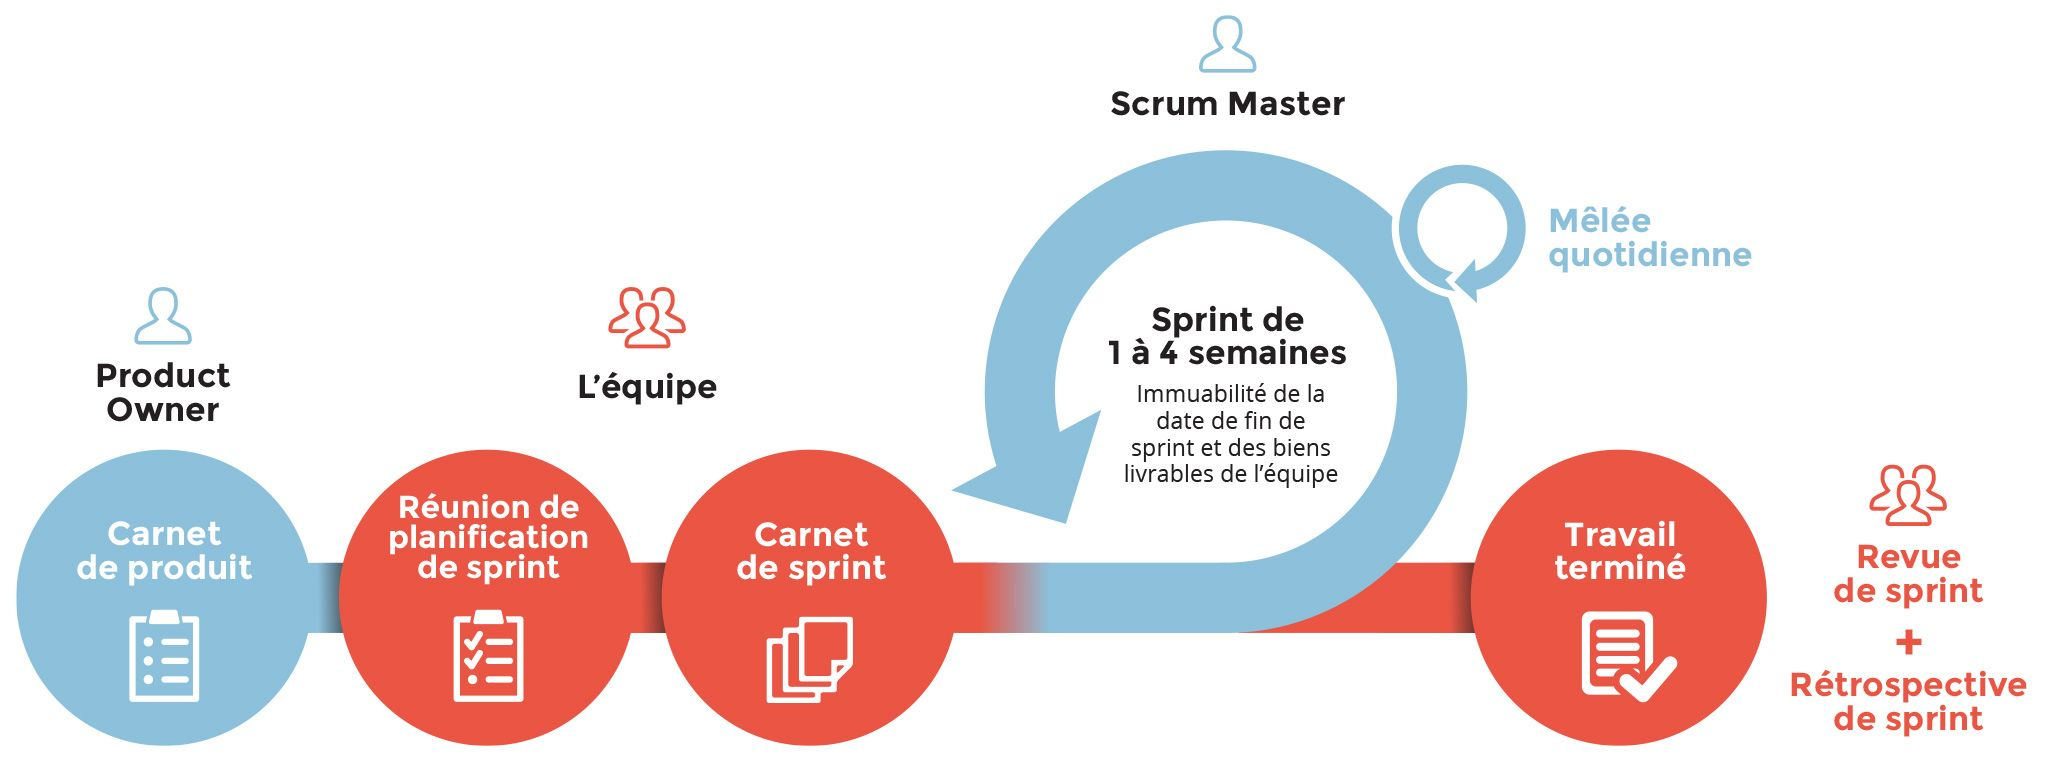
\includegraphics[width=1\textwidth]{img/capture1.jpeg}
    \caption{Cycle de vie du projet en mode agile}
    \label{fig:cycle}
\end{figure}




\newpage

\begin{ganttchart}{1}{12}
	\gantttitle{Durée en jours}{12} \\
	\gantttitlelist{1,...,12}{1} \\

	\ganttgroup{Groupe 1}{1}{7} \\ % elem0
	\ganttbar{Sujet 1a}{1}{4} \\ % elem1
	\ganttbar{Sujet 1b}{2}{7} \\ % elem2
	\ganttmilestone{Fin 1}{7} \\ % elem3
	\ganttlink{elem1}{elem3}
	\ganttlink{elem2}{elem3}

	\ganttgroup{Groupe 2}{8}{11} \\ % elem4
	\ganttbar{Sujet 2a}{8}{9} \\ % elem5
	\ganttbar{Sujet 2b}{10}{11} \\ % elem6
	\ganttmilestone{Fin 2}{11} \\ % elem7
	\ganttlink{elem5}{elem6}
	\ganttlink{elem6}{elem7}

	\ganttmilestone{Fin}{12} % elem8
	\ganttlink{elem3}{elem8}
	\ganttlink{elem7}{elem8}
\end{ganttchart}




\end{document}